\section{EXPLORATORY DATA ANALYSIS}
\label{sec:exploratory_analysis}

The final dataset comprises 64,119 flight records representing landing operations at Guarulhos International Airport (SBGR) collected between January and December 2025. The dataset includes temporal, operational, traffic, meteorological, and fuel-consumption-related variables. An exploratory data analysis (EDA) was conducted to investigate the distribution of KPI16 and its relationship with the explanatory variables, as well as identify relevant patterns and highlight relationships that might influence the additional fuel consumption (KPI16) in the terminal area.

The distribution of $kpi16$ presents elongated tails, as shown in Figure \ref{fig:kpi16-distribution}, indicating the presence of observations with significantly high additional consumption. Such cases may be associated with adverse operational conditions, such as airspace congestion, unfavorable weather, or prolonged holding procedures. Outlier analysis was handled conservatively, maintaining observations between the 1st and 99th percentiles to preserve extreme events that represent actual operational behavior within the system.

\begin{figure}[htbp]
    \centering
    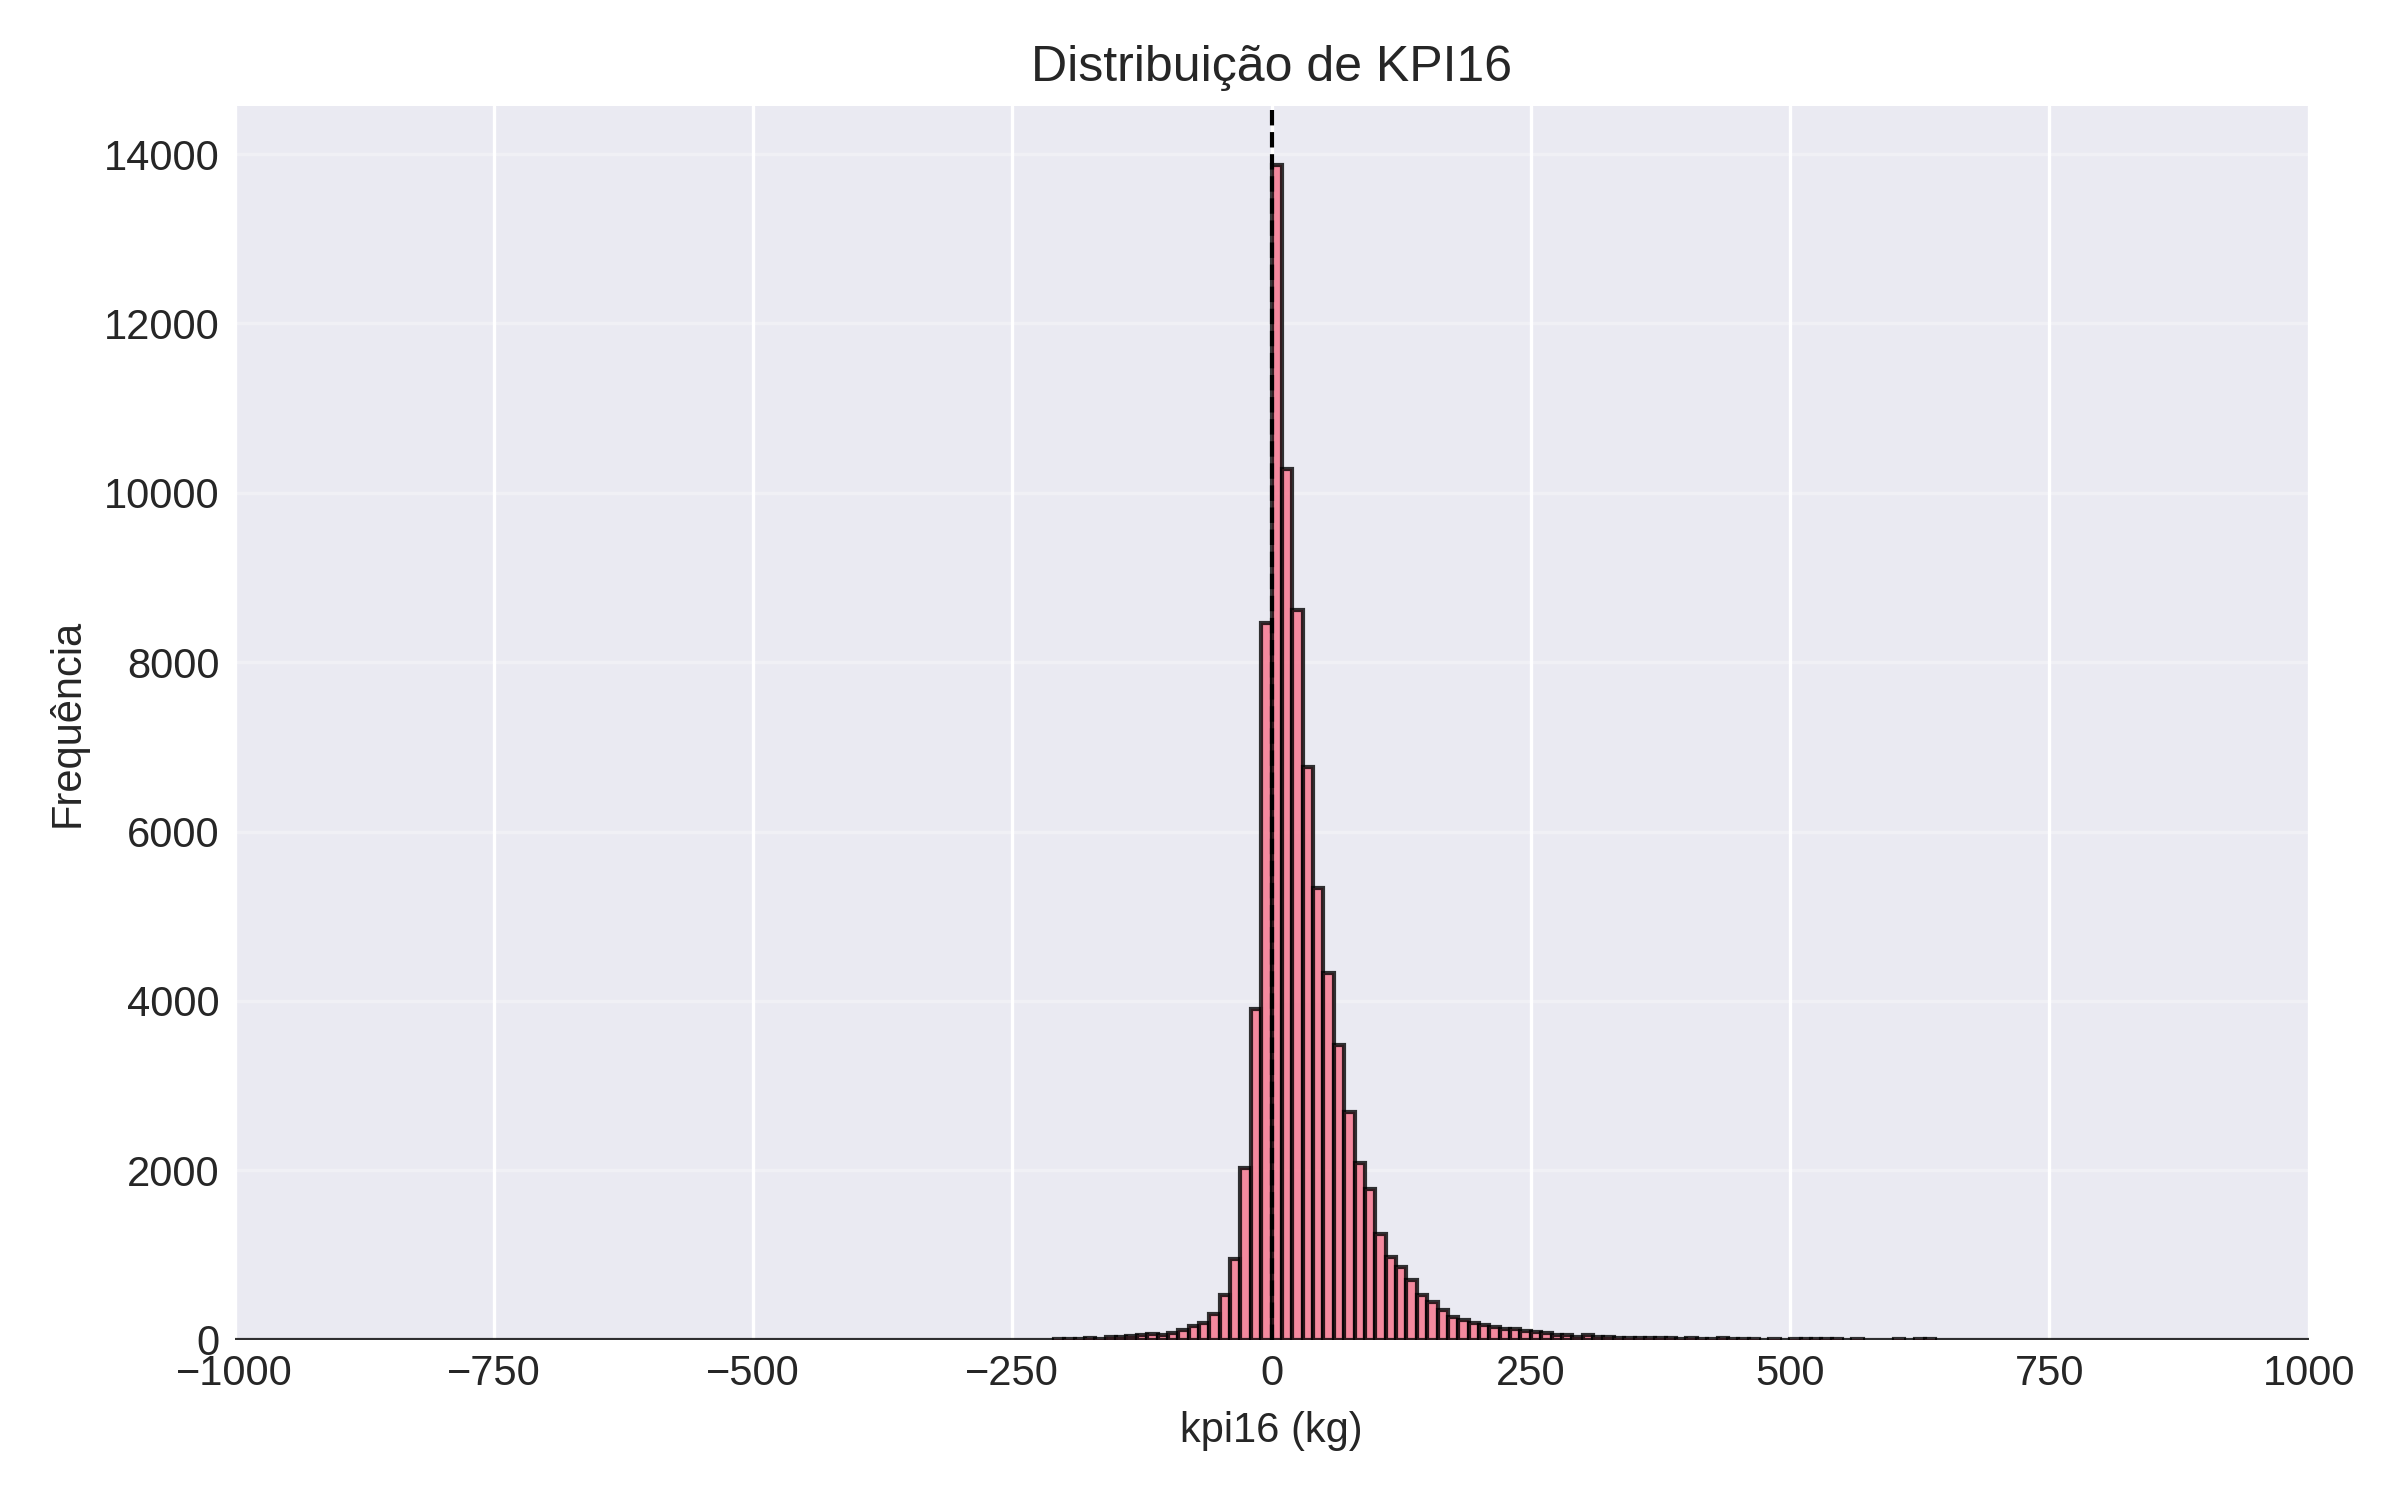
\includegraphics[width=1\linewidth]{images/kpi16-distribution.png}
    \caption{Distribution of the target variable $kpi16$ (Additional Fuel Consumption).}
    \label{fig:kpi16-distribution}
\end{figure}

\subsection{Additional Fuel Consumption by Departure Airport}
The departure airport (ADEP) plays a critical role in shaping the flight profile, cruise altitude, and approach procedure into the destination TMA. Figure \ref{fig:adep-kpi16} highlights the average additional fuel consumption (KPI16) for the 15 most frequent ADEPs. Notably, flights originating from Afonso Pena International Airport (SBCT) in Curitiba and Hercílio Luz International Airport (SBFL) in Florianópolis present the highest average penalties. This similarity indicates shared approach challenges, likely due to their geographical alignment and consequent entry routing into the Guarulhos TMA.

\begin{figure}[htbp]
    \centering
    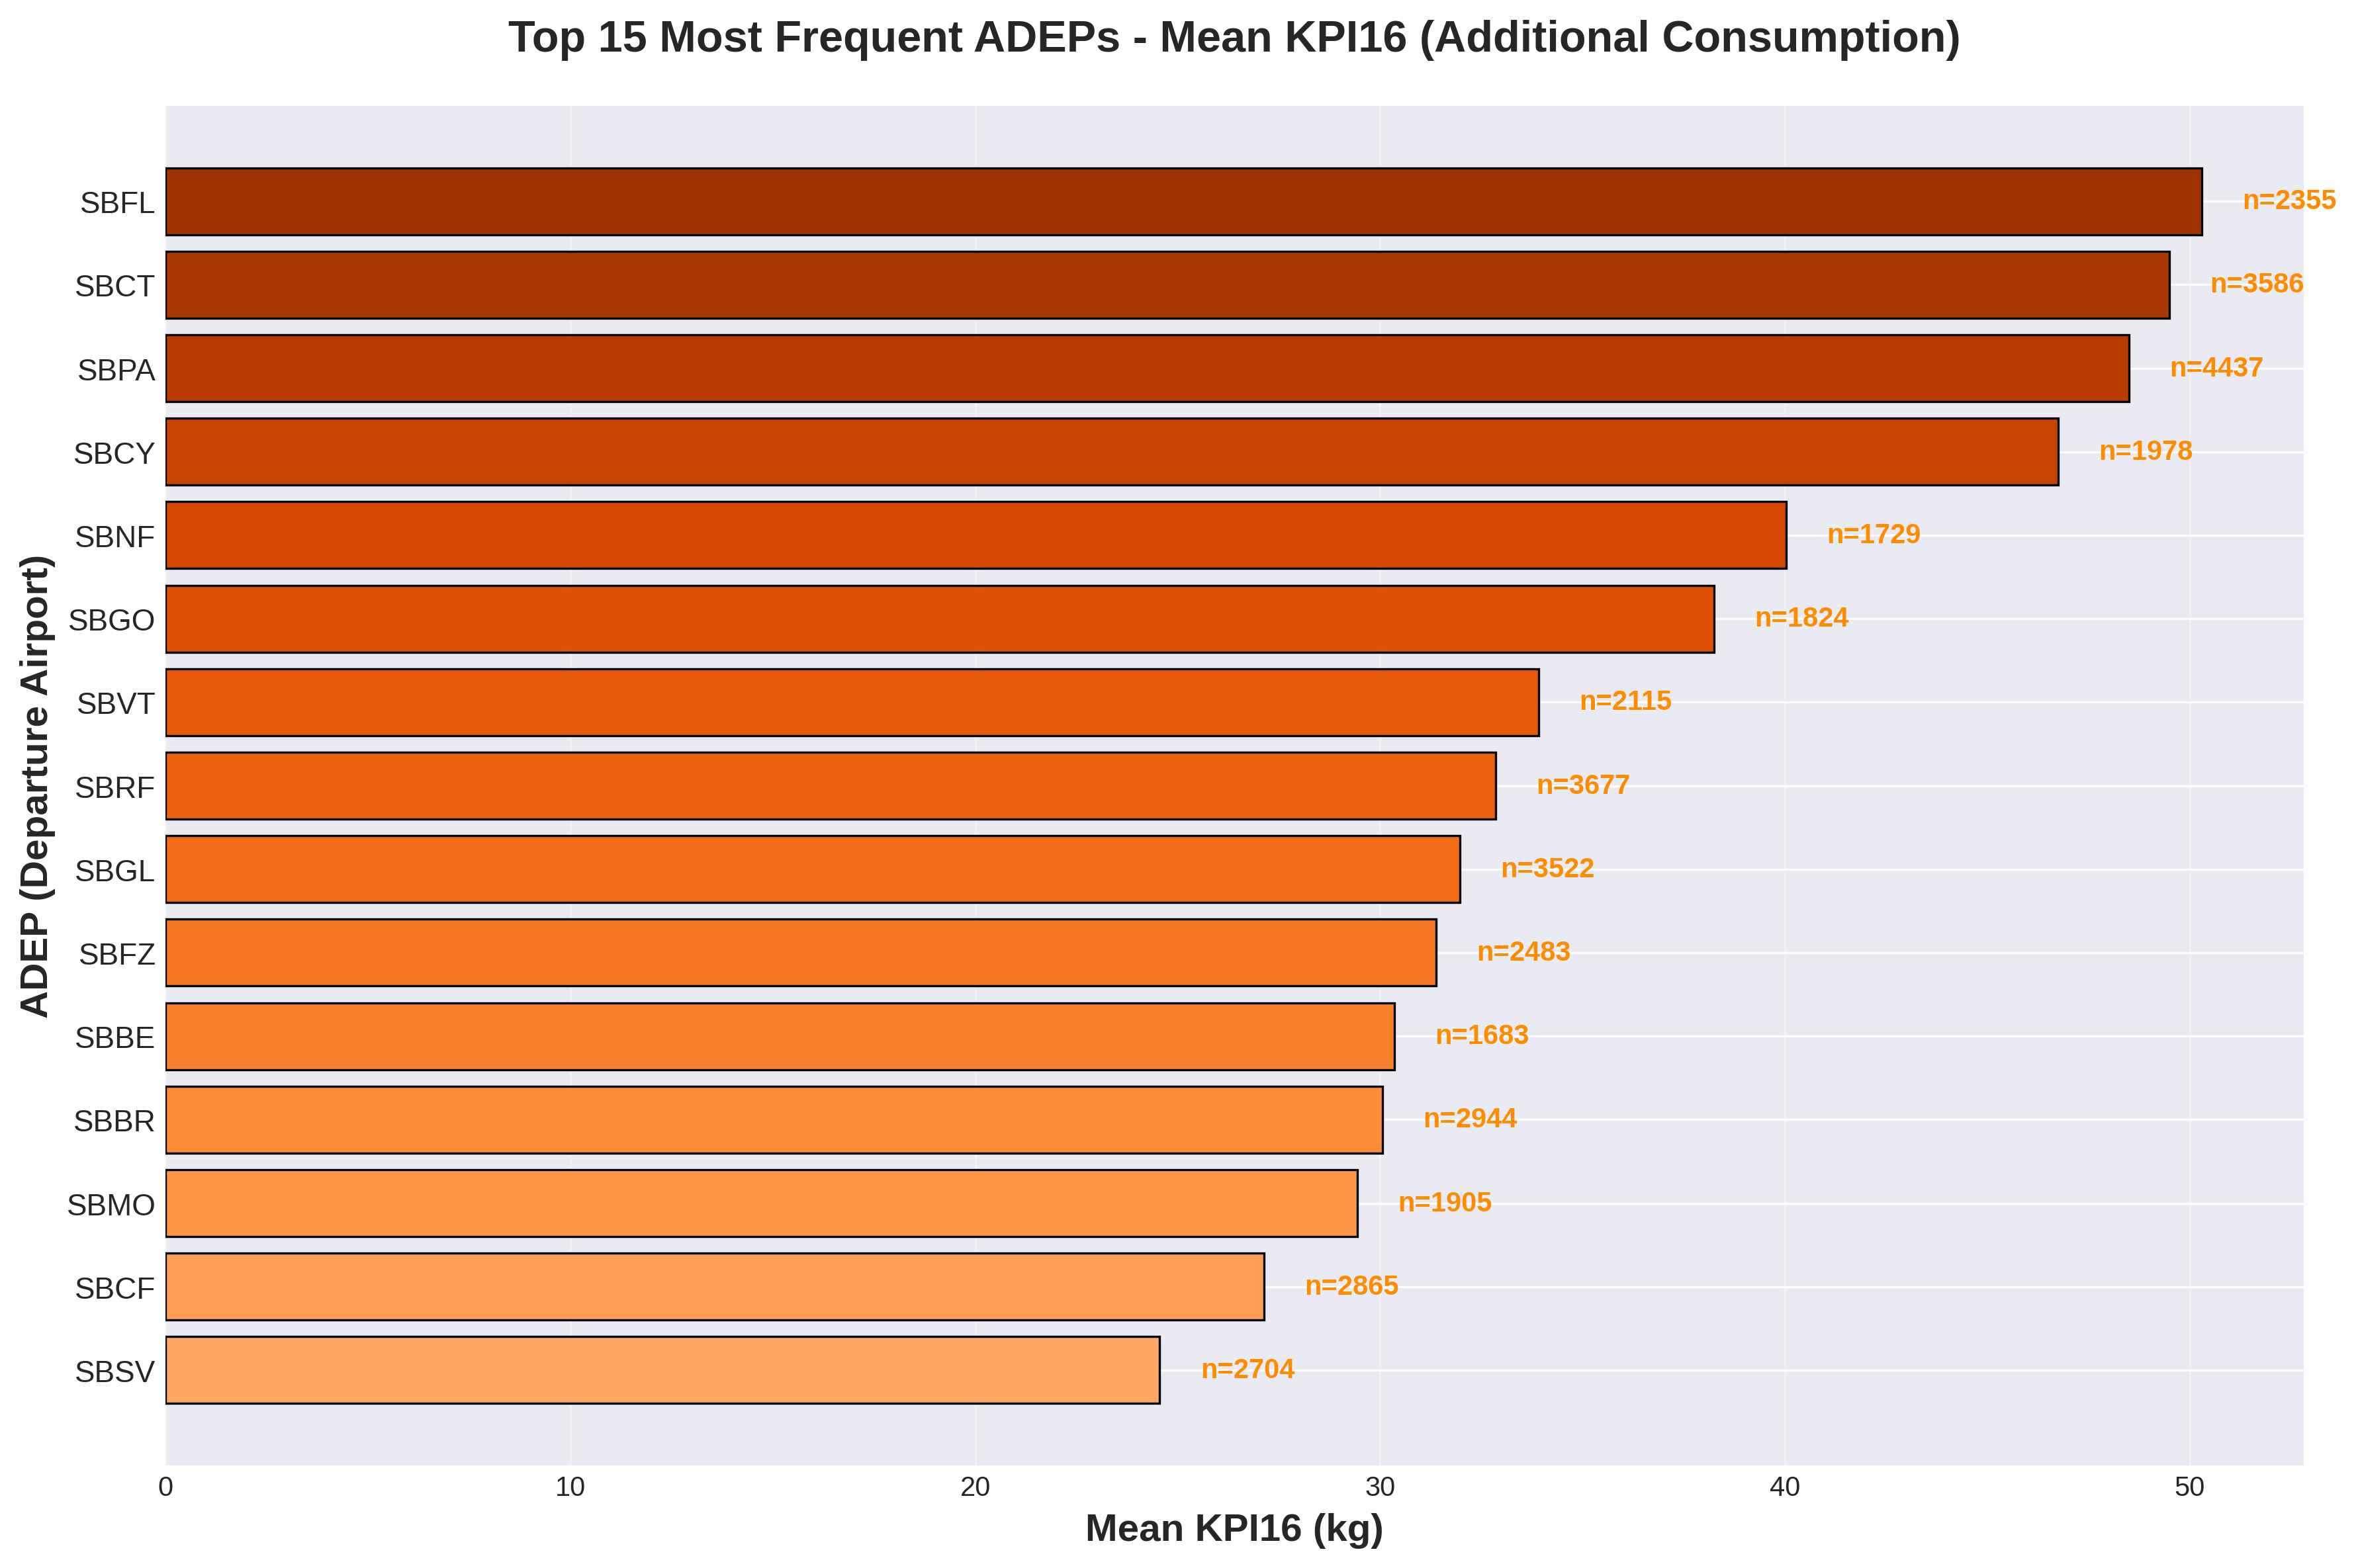
\includegraphics[width=1\linewidth]{images/adep_kpi16.png}
    \caption{Average additional fuel consumption (KPI16) by Departure Airport (ADEP).}
    \label{fig:adep-kpi16}
\end{figure}

\subsection{Impact of TMA Entry Sector on Efficiency}
To further investigate the geographical bottlenecks, the TMA was divided into entry sectors of 60-degree increments based on the aircraft's bearing upon crossing the terminal cylinder (excluding sector 120.0 due to insufficient sample size). As demonstrated in Figure \ref{fig:setor-kpi16}, flights entering through Sector 180.0 and Sector 300.0 demand the highest additional fuel consumption.

This pattern suggests that flights entering through these sectors may be associated with operational conditions that result in higher additional fuel consumption."

\begin{figure}[htbp]
    \centering
    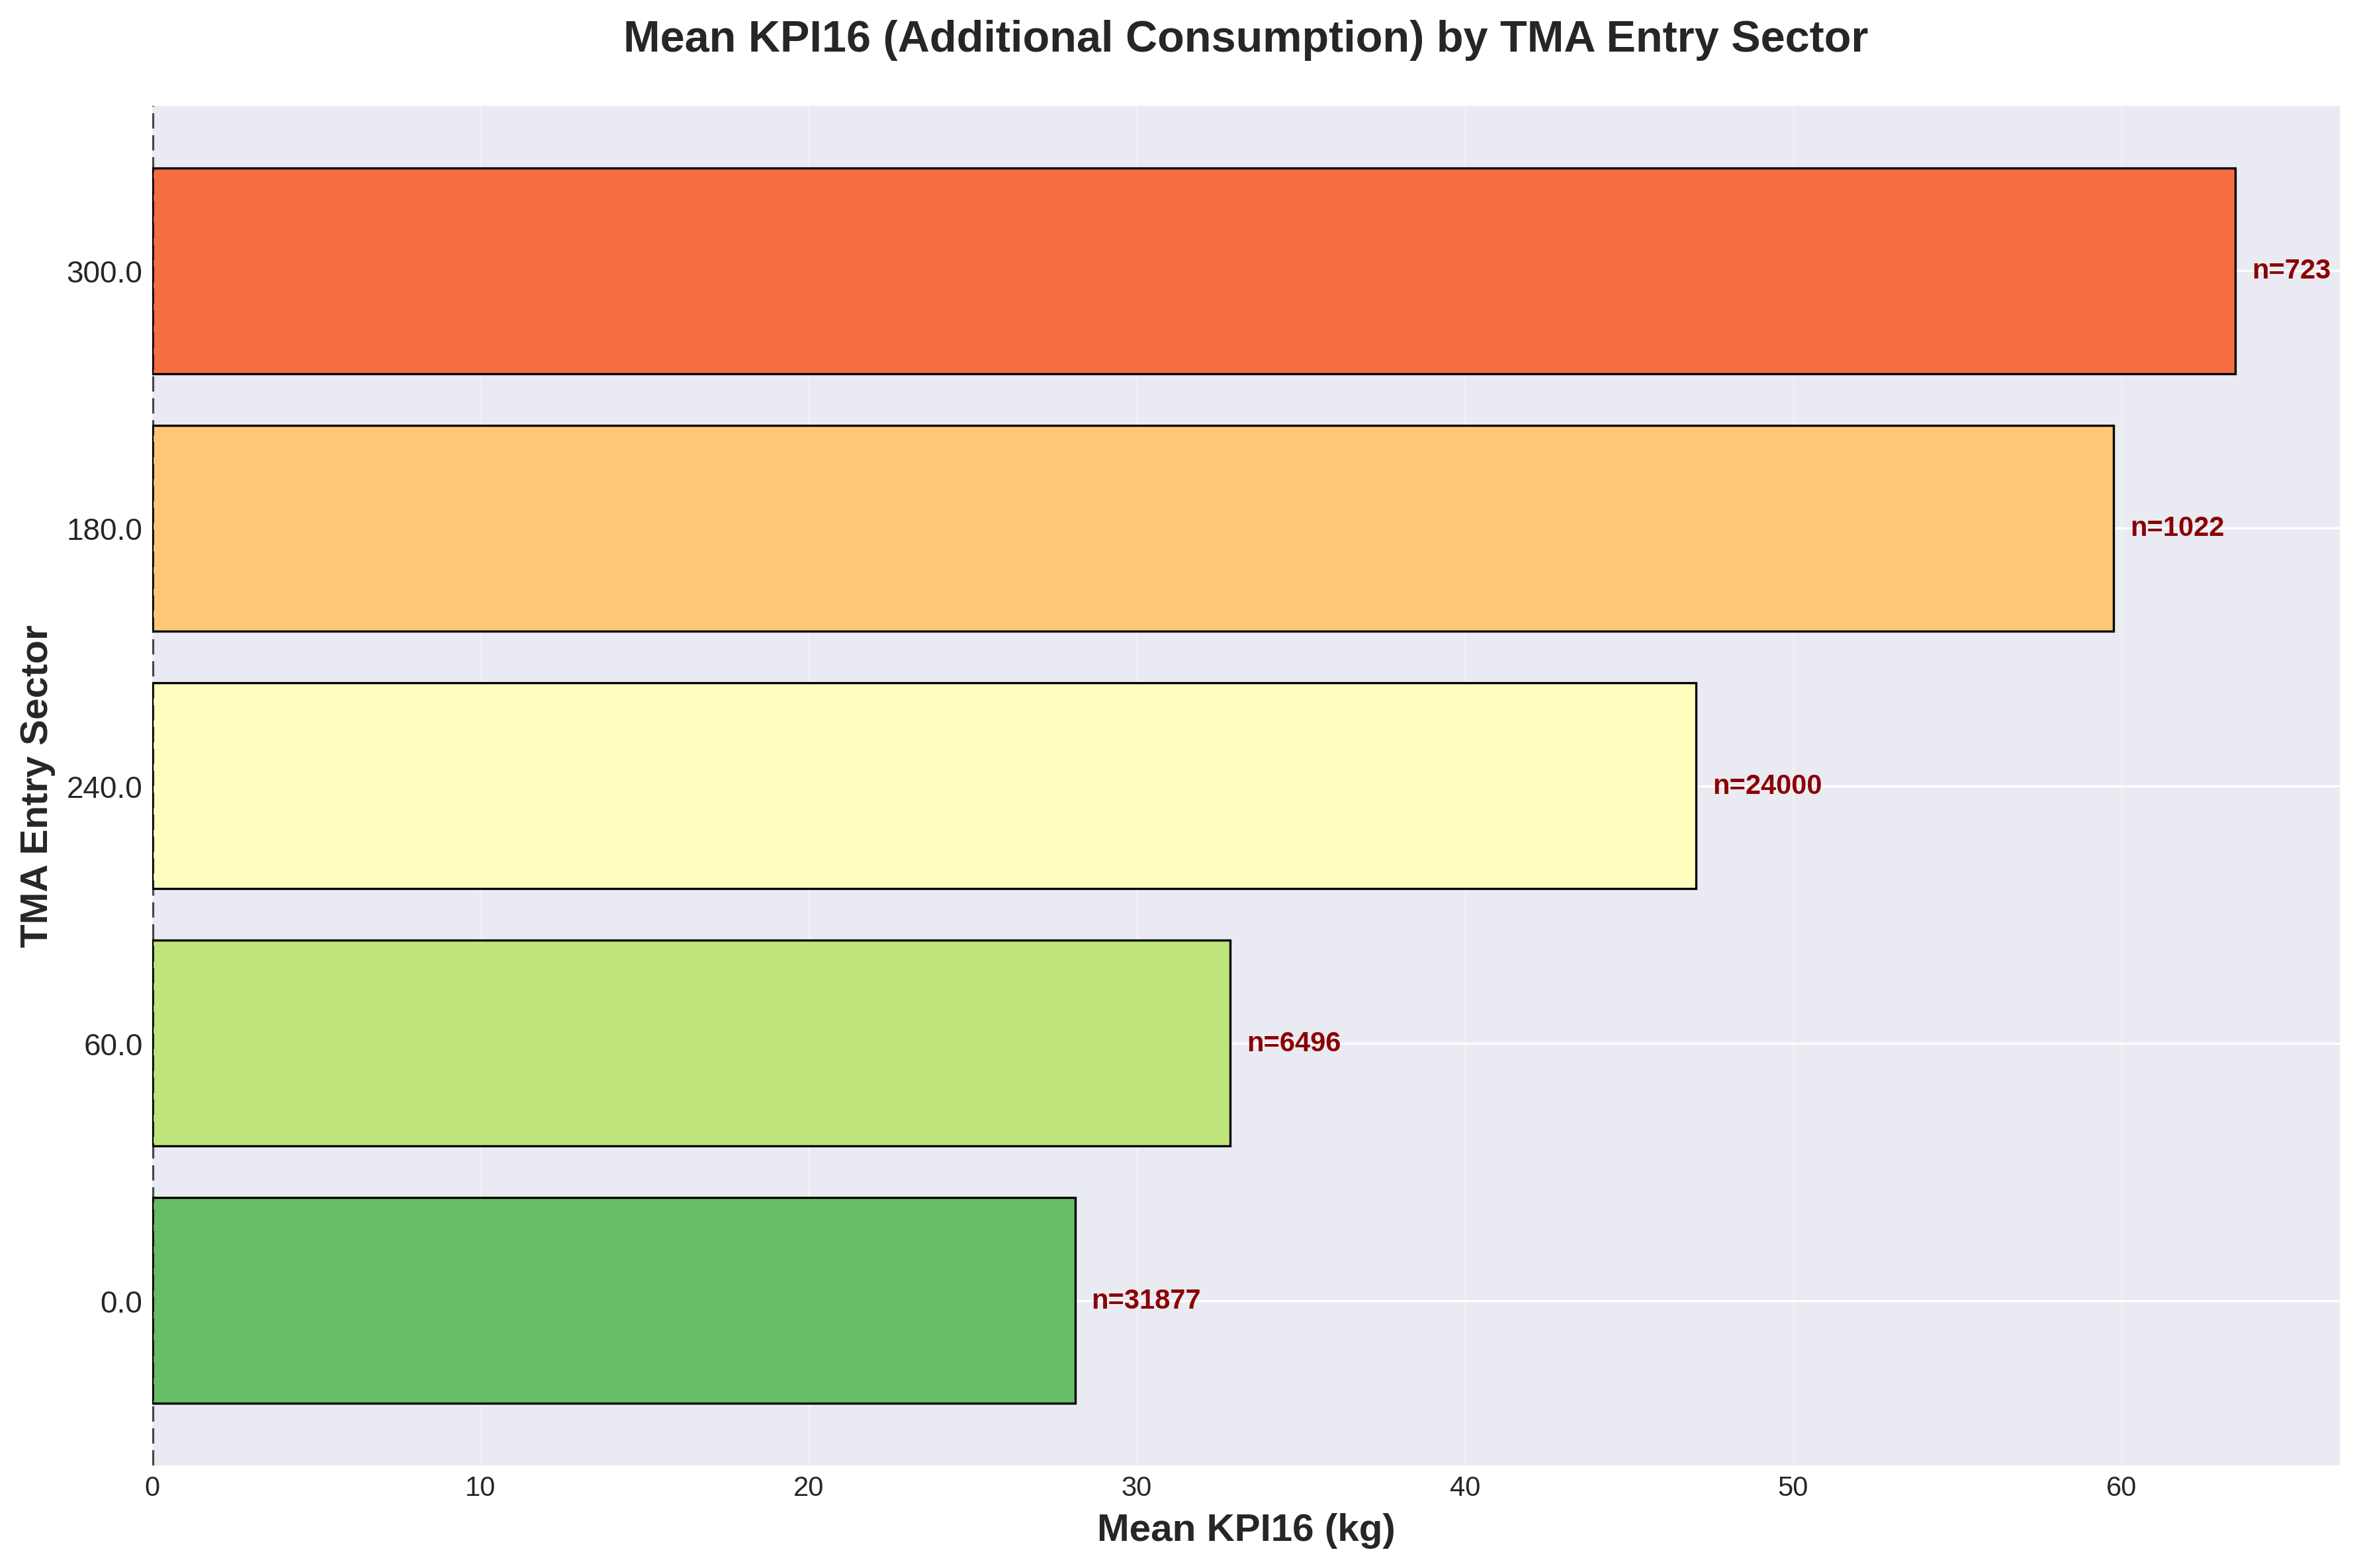
\includegraphics[width=1\linewidth]{images/setor_kpi16.png}
    \caption{Mean KPI16 (Additional Consumption) distributed by TMA Entry Sector.}
    \label{fig:setor-kpi16}
\end{figure}

\subsection{Interaction Between Entry Sectors and Origin Airports}
A more granular analysis combining both origin airports and entry sectors reveals the operational dynamics causing the aforementioned inefficiencies. Figure \ref{fig:setor-adep-kpi16} details the most frequent ADEPs for the most penalizing sectors. Sector 180.0 is predominantly saturated by flights from Southern capitals (Florianópolis, Porto Alegre, and Curitiba), while Sector 300.0 handles traffic from Goiânia, Uberlândia, and Manaus. The high additional consumption in these sectors suggests that flights arriving from these origins are frequently deprioritized or subjected to complex sequencing maneuvers due to concentrated traffic convergence.

\begin{figure}[htbp]
    \centering
    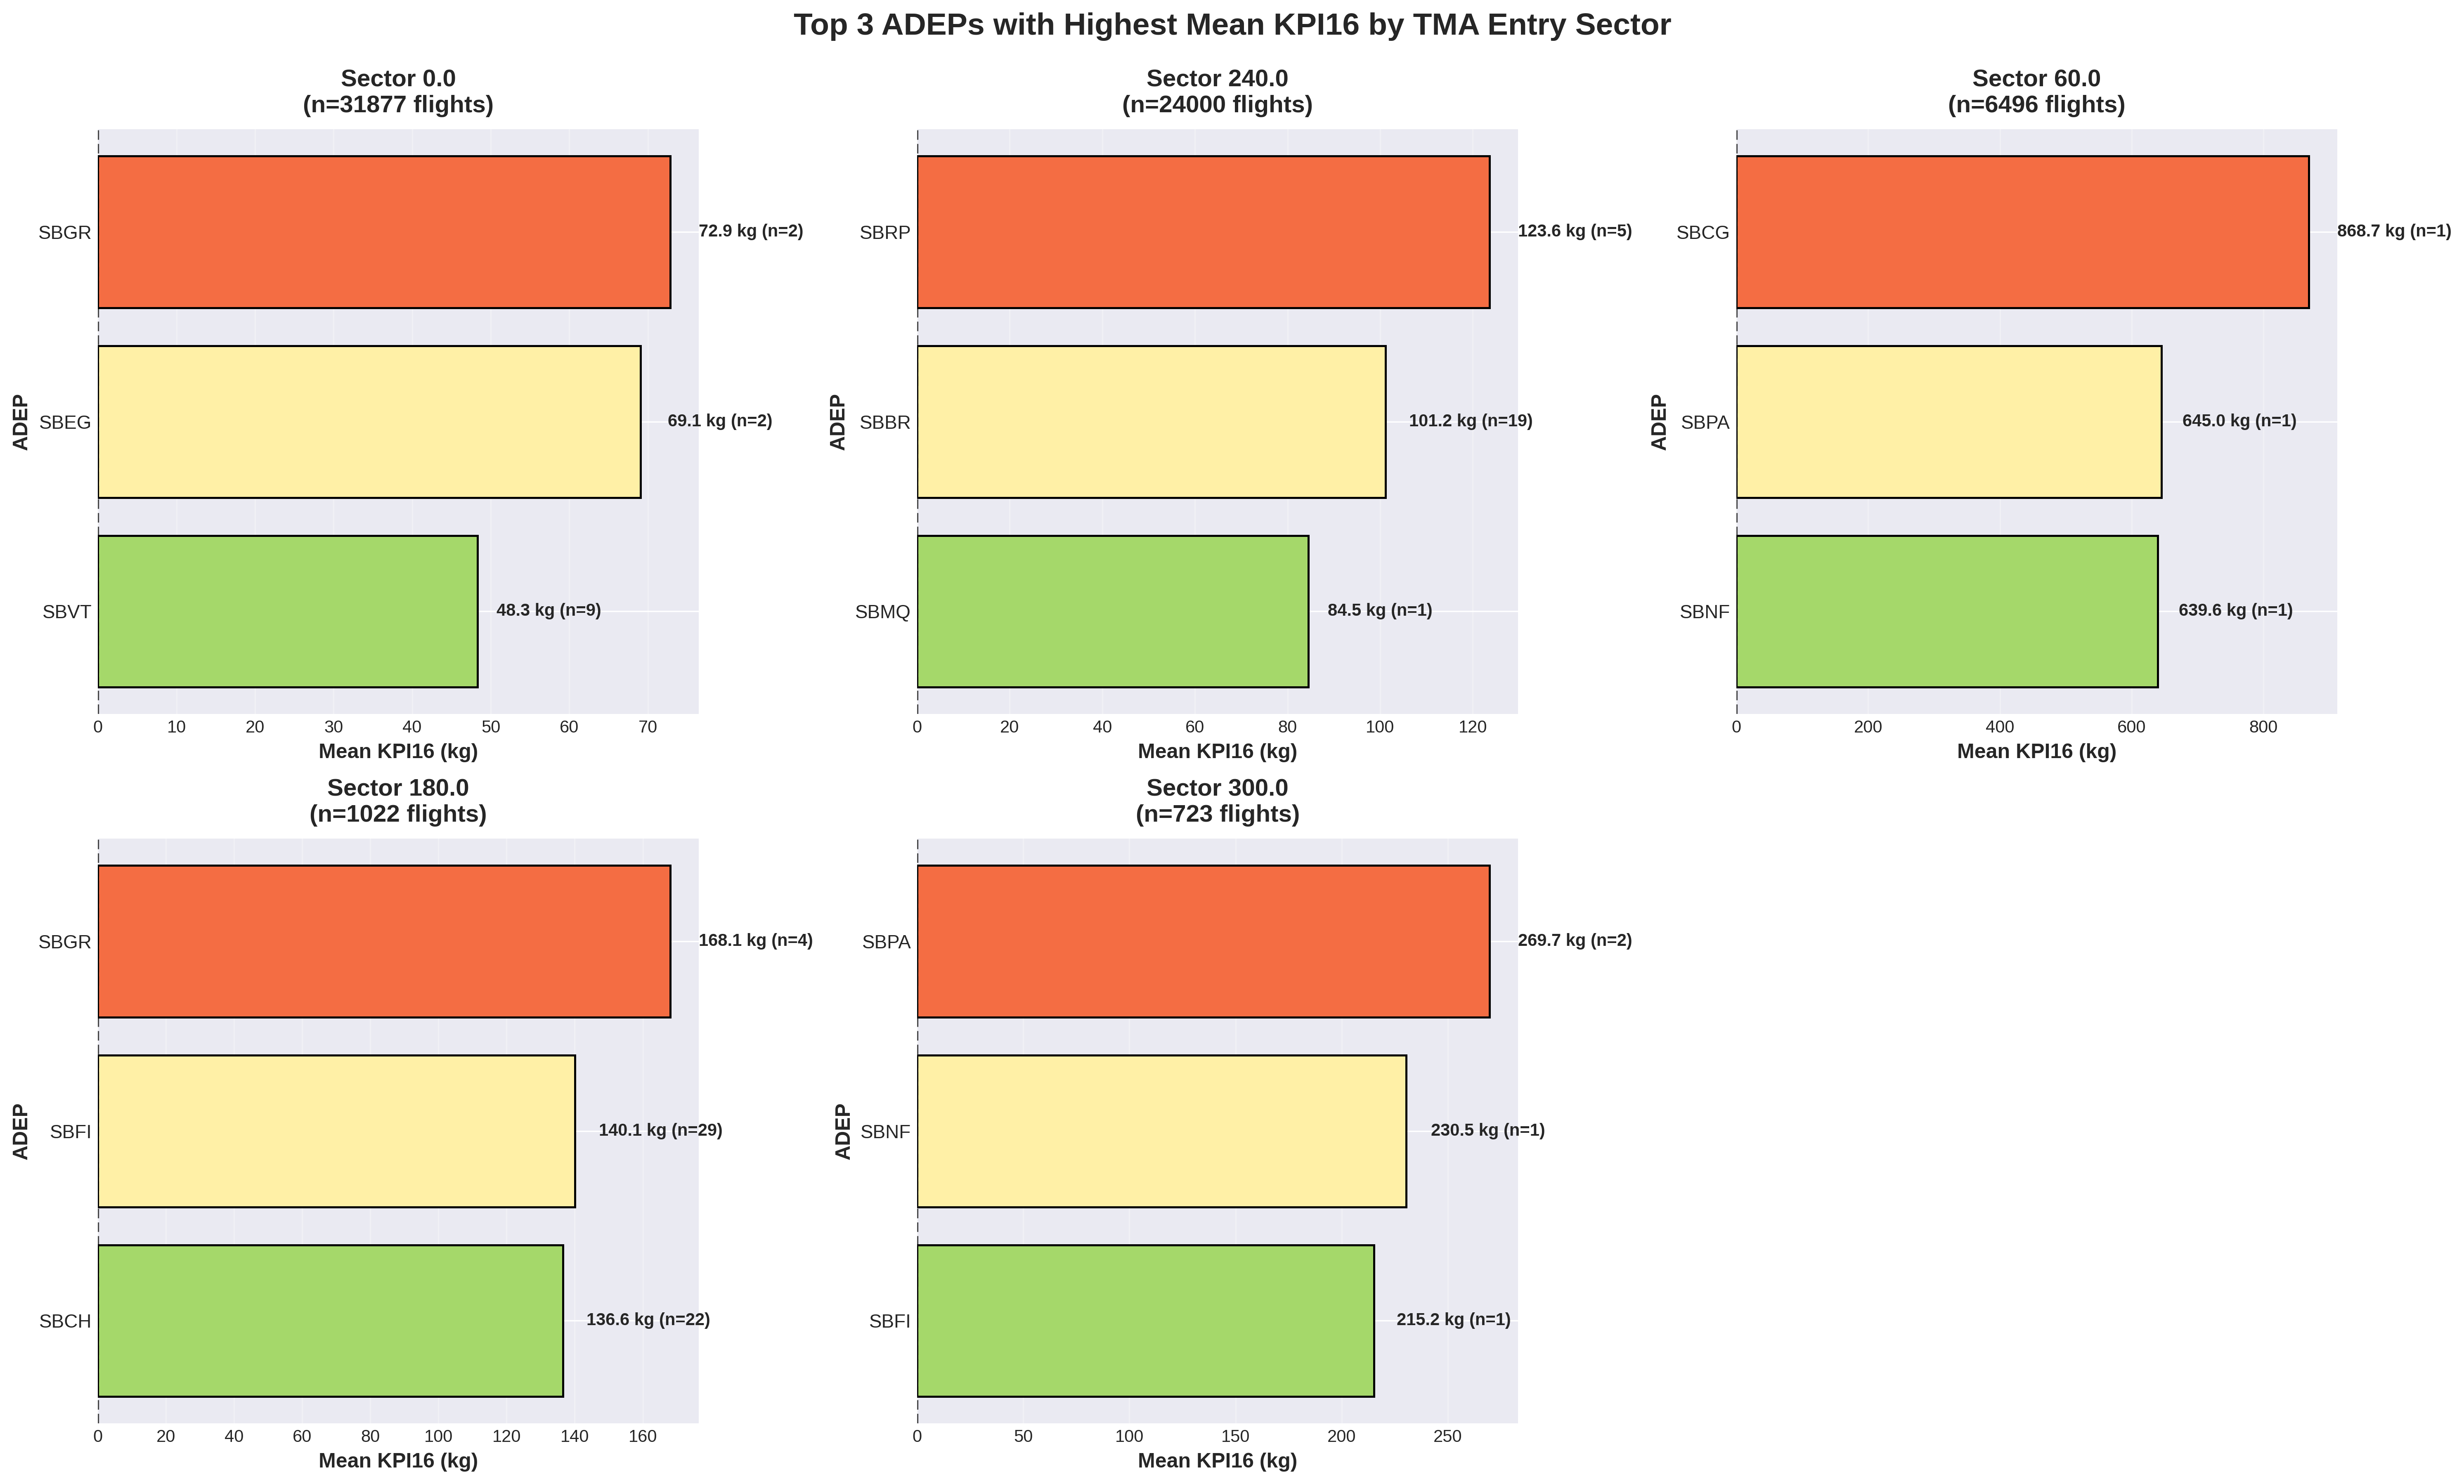
\includegraphics[width=1\linewidth]{images/setor_adep_kpi16.png}
    \caption{Top ADEPs contributing to high KPI16, grouped by TMA Entry Sector.}
    \label{fig:setor-adep-kpi16}
\end{figure}

\subsection{Hourly Traffic Variations and Congestion Cascading}
Air Traffic Control (ATC) is the service provided by ground-based air traffic controllers who direct aircraft on the ground and through controlled airspace to ensure safety and optimize traffic flow. Air traffic operates in waves, and the time of arrival heavily dictates the level of congestion encountered. Figure \ref{fig:hora-adep} groups the performance of the three most impactful ADEPs across the six busiest hours of the day. During these peak periods, Curitiba (SBCT) and Porto Alegre (SBPA) frequently alternate as the primary contributors to high KPI16. Because these flights saturate Sector 180.0 simultaneously, ATC is forced into heavy intervention, resorting to holding patterns and vectoring. Consequently, flights from Florianópolis (SBFL) sharing the same entry sector are often deprioritized, creating a cascading effect that explains its position as the airport with the highest overall average fuel penalty.

\begin{figure}[htbp]
    \centering
    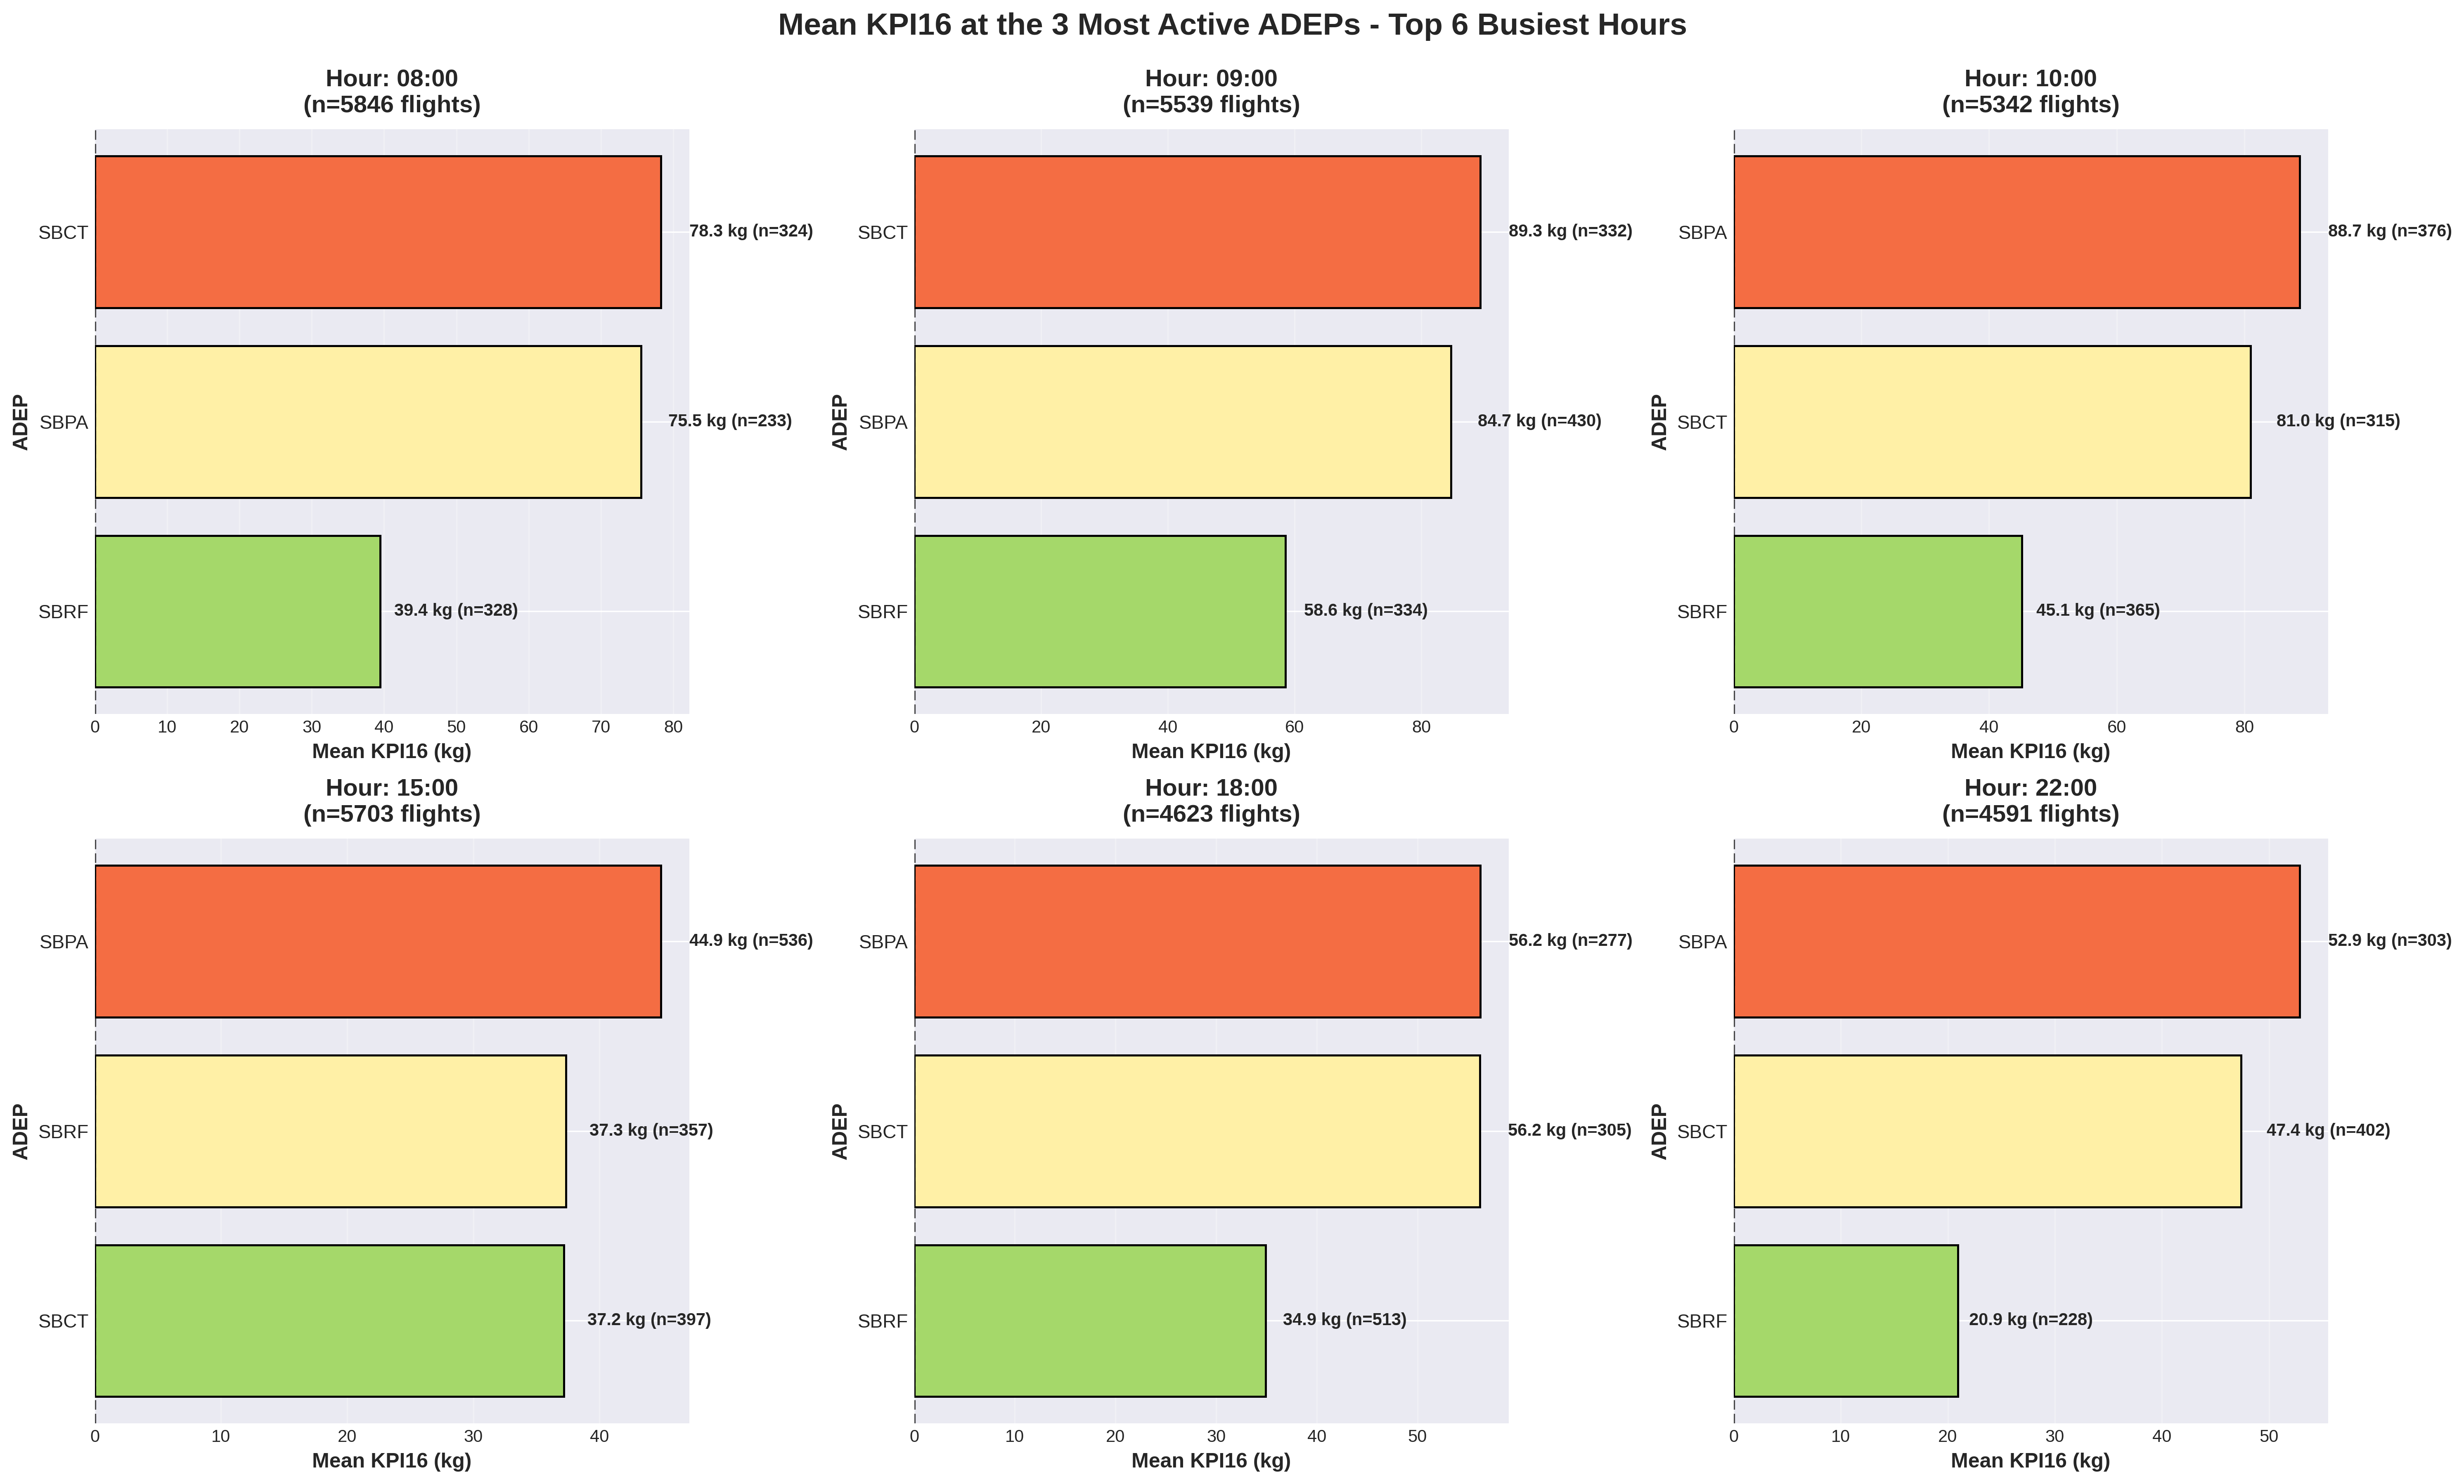
\includegraphics[width=1\linewidth]{images/hora_adep.png}
    \caption{Mean KPI16 for the three most active ADEPs during the top six busiest landing hours.}
    \label{fig:hora-adep}
\end{figure}